\documentclass[12pt, letterpaper]{article}
\usepackage[utf8]{inputenc}
\usepackage{amsmath}
\usepackage{parskip}

\usepackage{graphicx}
\graphicspath{{../images/}}

\usepackage{hyperref}
\hypersetup{
    colorlinks=true,
    urlcolor=blue,
    linkcolor=blue,
    citecolor=blue,
    filecolor=blue,
}
\urlstyle{same}

\title{Notes to Price Distribution}
\author{}
\date{}


\begin{document}

\maketitle

One key aspect of exploratory data analysis is investigating the \emph{distribution} of the outcome variable.
In our case the price distribution is highly right-skewed with a few very expensive listings pulling the mean and median of the price distribution further away from each other.

%%%
\begin{figure}[ht]
    \centering
    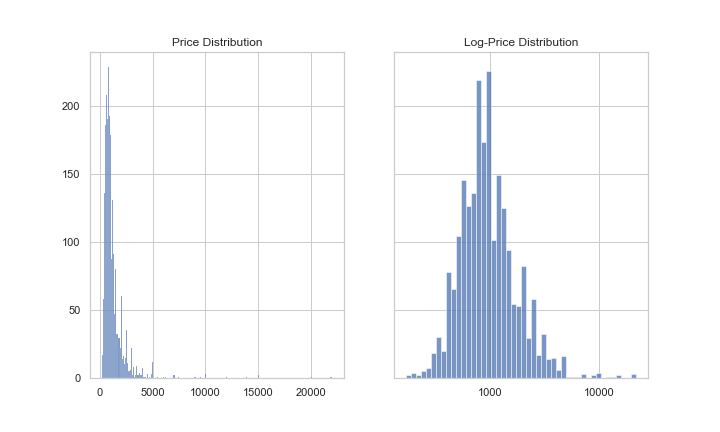
\includegraphics[width=0.8\textwidth]{price_distribution.png}
    \caption{Distribution of Apartment Prices on original and logarithmic Scale}
    \label{fig:price-distribution}
\end{figure}
%%%

Some statistical models such as \emph{Linear Regression} tend to perform better when the outcome distribution is symmetric and approximately normal, whereas some very flexible algorithms like \emph{Neural Networks} do not make any distributional assumptions and are capable of modeling any kind of distribution accurately.
Figure \ref{fig:price-distribution} illustrates an approximate normal distribution can be achieved with a simple logarithmic distribution.

Whereas \emph{all} of the classical models benefitted from the log-transformation resulting in lower error metrics, this was not the case for the Neural Network we used.

In fact, training turned out to be more challenging, since the \emph{magnitude} of the losses by comparing true and predicted price on the logarithmic scale was drastically reduced, leading to smaller gradients and thus smaller weight updates.
This issue could be mitigated to some extent with a larger learning rate.
However, in contrast to the untransformed version, the network still suffered from \emph{vanishing gradients} and \emph{loss plateaus}.

\newpage

\bibliography{bib}
\bibliographystyle{apalike}

\end{document}
